\PassOptionsToPackage{hyphens}{url}
\documentclass[sigconf,anonymous,review]{acmart}

% ACM Metadata & Rights Management Configuration
\settopmatter{printacmref=false} % Suppress ACM reference for review
\renewcommand\footnotetextcopyrightpermission[1]{} % Suppress copyright for review
\pagestyle{plain} % Insert page numbers for reviewers

% Mathematical and System Typographic Packages
\usepackage{amsmath,amsfonts}
\usepackage{booktabs}
\usepackage{subcaption}
\usepackage{microtype}
\usepackage{xspace}
\usepackage{balance}
\usepackage{multirow}

% TikZ & Plotting
\usepackage{tikz}
\usetikzlibrary{positioning, arrows.meta}
\usepackage{pgfplots}
\pgfplotsset{compat=1.18}

% Macro Definitions
\newcommand{\sysname}{\textsc{AdCausal}\xspace}
\newcommand{\cpm}{\text{CPM}\xspace}
\newcommand{\dcpm}{\Delta\cpm}
\newcommand{\etr}{\text{ETR}^*\xspace}
\newcommand{\etrinit}{\text{ETR}_{\text{initial}}\xspace}
\newcommand{\rid}{R_{\text{ID}}\xspace}
\newcommand{\htr}{\text{HTR}\xspace}
\newcommand{\ucost}{U_{\text{cost}}\xspace}

\usepackage{enumitem}
\setlist{nosep, leftmargin=*} 

% Compact spacing around figures, tables, and captions
\setlength{\textfloatsep}{5pt plus 1pt minus 1pt}
\setlength{\floatsep}{5pt plus 1pt minus 1pt}
\setlength{\intextsep}{5pt plus 1pt minus 1pt}
\setlength{\abovecaptionskip}{3pt plus 1pt minus 1pt}
\setlength{\belowcaptionskip}{3pt plus 1pt minus 1pt}

% Compact display equations
\setlength{\abovedisplayskip}{3pt plus 1pt minus 1pt}
\setlength{\belowdisplayskip}{3pt plus 1pt minus 1pt}

% 1. Emergency stretch: Forces LaTeX to wrap lines instead of spilling into margins
\emergencystretch=3em
\hfuzz=1pt % Ignores tiny sub-1pt overflows that human eyes cannot see

% 2. Enable hyphenation inside \texttt (LaTeX disables it by default)
\usepackage[htt]{hyphenat}

% 3. Allow inline math to break across lines at operators (=, \ge, +, etc.)
\binoppenalty=700
\relpenalty=500

% Anonymous Review Header
\acmConference[Review Submission]{The Web Conference (WWW)}{Double-Blind Review Copy}{Confidential}
\acmYear{2027}

\begin{document}

\title{A Causal Measurement of Anti-Fingerprinting Defense Effectiveness in the Real-World Ad Ecosystem}

% Double-blind author block
\author{Anonymous Author(s)}
\affiliation{
  \institution{Double-Blind Submission to The Web Conference (WWW)}
  \country{}
}
\email{}

% Abstract
\begin{abstract}
Third-party cookie deprecation and client-side storage partitioning have accelerated the commercial deployment of stateless browser fingerprinting across programmatic advertising ecosystems. Existing empirical benchmarks evaluate anti-fingerprinting defenses through passive script detection or synthetic Shannon entropy calculations—metrics that capture tracking intent or theoretical variance, but fail to establish whether defenses prevent client re-identification in production ad tech.

In this work, we present the first outcome-oriented, causal measurement framework that leverages programmatic Real-Time Bidding (RTB) clearing prices as an empirical economic oracle for identity certainty. Deploying an automated infrastructure across 150 commercial publishers under native browser execution, we enforce a three-phase intervention: training high-intent behavioral profiles, capturing baseline Prebid.js bids, purging all client-side stateful storage, and measuring post-purge bid trajectories across five hardened and baseline browser configurations.

Our framework reveals that stateful clearing alone is completely ineffective: unhardened Google Chrome exhibits an unperturbed median bid shift of $-1.12\%$ ($p = 0.4832$, Re-ID rate $R_{\text{ID}} = 0.606$), proving commercial Demand-Side Platforms (DSPs) seamlessly bridge storage resets via stateless fingerprints. Conversely, anti-fingerprinting defenses construct an empirical Pareto frontier. Hardened Mozilla Firefox (combining RFP normalization with state partitioning) emerges as a zero-cost defense, yielding a $-26.87\%$ median bid collapse ($p = 0.0734$) with zero runtime exception overhead ($U_{\text{cost}} = 0.00$). Hardened Brave Browser achieves the apex of tracking disruption ($-59.97\%$ median collapse, $R_{\text{ID}} = 0.500$), but imposes a $+44\%$ increase in runtime script breakage ($U_{\text{cost}} = 0.44$).

Finally, we deconstruct the ``Usability Trap''—showing how defensive network blocking triggers tracker retry loops that distort naive tracking metrics—and formulate the Refined Effectiveness-to-Risk metric ($\text{ETR}^*$), providing a mathematically robust benchmark for privacy-preserving web engineering.
\end{abstract}

% CCS Concepts & Keywords (WWW Requirement)
\begin{CCSXML}
<ccs2012>
   <concept>
       <concept_id>10002978.10003029.10011703</concept_id>
       <concept_desc>Security and privacy~Usability in security and privacy</concept_desc>
       <concept_significance>500</concept_significance>
   </concept>
   <concept>
       <concept_id>10002978.10003014.10003015</concept_id>
       <concept_desc>Security and privacy~Web protocol security</concept_desc>
       <concept_significance>500</concept_significance>
   </concept>
   <concept>
       <concept_id>10002951.10003260.10003282</concept_id>
       <concept_desc>Information systems~Web applications</concept_desc>
       <concept_significance>300</concept_significance>
   </concept>
 </ccs2012>
\end{CCSXML}

\ccsdesc[500]{Security and privacy~Usability in security and privacy}
\ccsdesc[500]{Security and privacy~Web protocol security}
\ccsdesc[300]{Information systems~Web applications}

\keywords{Browser Fingerprinting, Web Privacy, Real-Time Bidding, Causal Inference, Programmatic Advertising}

\maketitle

% Core Body Sections (Pages 1-8: Must be self-contained)
\section{Introduction}
\label{sec:intro}

For two decades, the commercial web's surveillance economy operated on stateful storage primitives: HTTP cookies, Flash Local Shared Objects, and HTML5 Web Storage~\cite{eckersley2010panopticlick, englehardt2016openwpm}. In response to consumer pushback and regulatory mandates, major browser vendors introduced storage partitioning architectures, notably Apple WebKit's Intelligent Tracking Prevention (ITP) and Mozilla Gecko's Total Cookie Protection (dFPI). As third-party cookies decay, tracking consortiums have systematically pivoted to \textbf{stateless browser fingerprinting}: interrogating hardware, driver, and OS-level attributes through Web APIs (Canvas, WebGL, AudioContext, WebRTC, and system font enumeration) to reconstruct persistent cross-site behavioral graphs~\cite{laperdrix2016amiunique, iqbal2021fpinspector}.

To counteract stateless tracking, modern browsers deploy two fundamentally diverging anti-fingerprinting philosophies:
\begin{enumerate}
    \item \textbf{API Normalization:} Emulated by Tor Browser and Mozilla's Resist Fingerprinting (\texttt{privacy.resistFingerprinting}, RFP), which quantizes high-resolution timers, spoofs system attributes to standardized pools, and forces canvas readbacks to uniform white screens to maximize client anonymity sets~\cite{demir2022reproducibility}.
    \item \textbf{API Randomization (Farbling):} Implemented by Brave Browser, which injects cryptographically pseudo-random, session-ephemeral noise into canvas rendering, audio buffers, and hardware device enumeration, ensuring that subsequent readbacks generate divergent hashes that disrupt cross-session linking~\cite{liu2025fptrace}.
\end{enumerate}

Despite these deployments, the measurement literature lacks a rigorous methodology to determine whether these defenses functionally protect users in production. Current empirical benchmarks suffer from two structural flaws:

\paragraph{The Intent vs. Outcome Fallacy}
Passive measurement platforms (e.g., OpenWPM~\cite{englehardt2016openwpm}, FP-Inspector~\cite{iqbal2021fpinspector}) instrument JavaScript APIs to log when heuristic execution patterns occur. While effective for detecting tracking *intent*, observing a canvas readback provides zero verification of tracking *success*. It cannot determine whether the extracted payload resolved a user within an ad-tech identity graph or failed to overcome environmental noise.

\paragraph{The Theoretical Entropy Gap}
Synthetic benchmarks (e.g., Panopticlick~\cite{eckersley2010panopticlick}, AmIUnique~\cite{laperdrix2016amiunique}) benchmark defenses by calculating the Shannon entropy bits subtracted from isolated Web APIs. However, theoretical entropy reductions do not guarantee tracking severance in the wild. If an advertising network combines a partially farbled canvas signature with residual cross-site signals, such as IP-range localization, TLS client fingerprints, and User-Agent headers. Client re-identification persists despite nominal entropy loss.

\paragraph{Real-Time Bidding as an Economic Oracle}
To overcome the limitations of proxy measurements, we exploit a direct side-channel oracle: \textbf{programmatic Real-Time Bidding (RTB) clearing prices}~\cite{liu2025fptrace}. In header bidding auctions orchestrated via client-side Prebid.js wrappers, algorithmic Demand-Side Platforms (DSPs) submit bids (Cost Per Mille, or \cpm) within milliseconds based on identity certainty~\cite{pachilakis2019imc}. Econometric studies establish that an identified user commanding a rich cross-site behavioral profile sells for a $30\%$ to $60\%+$ valuation premium over an untargeted contextual impression~\cite{beales2014navigant, johnson2020marketsci, google2019cookies}. 

When an anti-fingerprinting defense successfully breaks cross-site tracking across an enforced stateful reset, DSP identity graphs are severed. Lacking identity certainty, bidding algorithms retreat to contextual reserve floors, precipitating a measurable collapse in \cpm clearing prices.

\paragraph{Contributions}
To quantify this phenomenon, we built a cluster-scale causal measurement platform that drives native Linux browser binaries across 150 commercial publishers. Our work delivers four primary contributions:
\begin{itemize}
    \item \textbf{Causal Measurement Methodology:} We design a 3-phase experimental protocol that trains high-intent personas, records pre-break ad-auction baselines, programmatically purges stateful storage, and measures post-purge economic bid shifts, causally isolating stateless tracking in the wild.
    \item \textbf{Validation of the Negative Control:} We demonstrate that in unhardened Google Chrome, stateful storage purges yield a negligible bid shift of only \textbf{$-1.12\%$} ($p = 0.4832$, fail to reject $H_0$). This provides empirical proof that clearing cookies without anti-fingerprinting defenses is entirely futile against commercial ad tech.
    \item \textbf{The Empirical Pareto Frontier:} We characterize an operational trade-off in browser engineering: \textit{Hardened Firefox} achieves the \textbf{Stealth / Zero-Breakage Optimum} ($-26.87\%$ median bid collapse, $p = 0.0734$, with zero usability breakage: $\ucost = 0.00$); whereas \textit{Hardened Brave} reaches the \textbf{Maximum Privacy Optimum} ($-59.97\%$ median collapse, $\rid = 0.500$), but imposes a $+44\%$ increase in runtime script exceptions ($\ucost = 0.44$).
    \item \textbf{Deconstructing the Usability Trap \& Metric Refinement:} We show that defensive request blocking triggers tracker retry loops ($28,976$ requests in Firefox Hardened) that invert naive evaluation metrics. We formalize the Refined Effectiveness-to-Risk metric ($\etr$), resolving structural pathologies and restoring monotonic rigor to privacy defense evaluation.
\end{itemize}
\section{Background \& Threat Model}
\label{sec:background}

\subsection{Programmatic Advertising \& Header Bidding}
Modern web publishers monetize digital inventory via programmatic Real-Time Bidding (RTB)~\cite{castelluccia2014selling, bashir2016tracing}. 
While legacy display monetization relied on monolithic waterfall ad servers (e.g., Google Ad Manager), modern publishers deploy \textbf{Header Bidding} wrappers, principally the open-source \texttt{Prebid.js} framework, embedded directly in the client-side DOM to conduct parallel auctions prior to ad-server calls~\cite{pachilakis2019no, cook2020inferring}.

When a client navigates to a publisher, the programmatic auction resolves through four sequential stages~\cite{pachilakis2019no, barysei2023investigating}:
\begin{enumerate}
    \item \texttt{Prebid.js} reads configuration tags, identifies active ad slots, and dispatches parallel, asynchronous HTTP bid requests to configured Supply-Side Platform (SSP) adapters (e.g., Rubicon, OpenX, AppNexus)~\cite{cook2020inferring};
    \item Each SSP adapter forwards the bid request via OpenRTB protocols to participating Demand-Side Platforms (DSPs), encapsulating client attributes: geographic IP localization, viewport dimensions, historical cookie-synchronization tokens~\cite{papadopoulos2019cookie}, smuggled navigational identifiers~\cite{randall2022measuring}, and stateless device fingerprint hashes extracted by embedded scripts~\cite{papadogiannakis2021user};
    \item DSP bidding algorithms parse the payload and query internal identity graphs: matching an affluent persona triggers aggressive premium bidding (\$2.50--\$15.00 CPM), whereas unresolved identities retreat to generic contextual reserve floors (\$0.05--\$0.25 CPM)~\cite{barysei2023investigating};
    \item Winning bids return to the browser, where \texttt{Prebid.js} resolves the highest clearing \cpm, surfaces it to the publisher's ad server, and renders the winning creative inside an isolated \texttt{iframe}.
\end{enumerate}

\subsection{The Economic Targeting Premium}
\label{subsec:targeting_premium}

The foundation of programmatic digital advertising is that identified users command significantly higher clearing prices than un-profiled users~\cite{castelluccia2014selling, bashir2016tracing}. Longitudinal empirical analysis by Beales and Eisenach established that behavioral-targeted advertising sells for a $2.68\times$ price premium over non-targeted contextual advertising ($+168\%$)~\cite{beales2014empirical}. 

Subsequent field trials by Google confirmed that stripping user identifiers decreases publisher ad revenue by an average of $52\%$~\cite{google2019cookie}, an empirical finding corroborated by Johnson et al., who documented an identical $52\%$ ad revenue loss when consumers opt out of behavioral profiling~\cite{johnson2020consumer}. 

Consequently, we formalize auction clearing \cpm as an \textit{economic side-channel oracle}:
\begin{equation}
\cpm(u) = \alpha \cdot \mathbb{I}_{\text{identified}}(u) + \beta_{\text{context}} + \epsilon_{\text{market}}
\label{eq:economic_oracle}
\end{equation}
where $\alpha$ represents the behavioral targeting premium ($\alpha > 0$)~\cite{beales2014empirical, johnson2020consumer}, $\beta_{\text{context}}$ represents baseline contextual inventory value, and $\epsilon_{\text{market}}$ denotes stochastic auction noise driven by DSP pacing algorithms and exchange latency~\cite{barysei2023investigating}.

\subsection{Threat Model}
\label{subsec:threat_model}

\paragraph{Adversarial Capabilities}
We model commercial tracking consortiums, SSPs, and DSPs under the classical \textbf{honest-but-curious} (semi-honest) adversarial model operating across the programmatic advertising mesh~\cite{papadopoulos2019cookie, oh2022cart}. 
The adversary operates within standard unprivileged client execution contexts, possessing legitimate access to standard DOM and Web APIs~\cite{bujlow2017survey, laperdrix2020browser}. 
Embedded third-party scripts participate in header bidding auctions and attempt to persist user identities across disjoint first-party administrative domains ($s_i \neq s_j$) without user consent~\cite{papadogiannakis2021user}. 

The adversary leverages standard stateless fingerprinting vectors documented in the literature: Canvas pixel extraction~\cite{mowery2012pixel, acar2014web}, WebGL parameter enumeration~\cite{cao2017cross}, AudioContext oscillator decay~\cite{englehardt2016openwpm, laperdrix2020browser}, clock skew timing attacks~\cite{sanchez2018clock}, browser extension profiling~\cite{starov2019unnecessarily}, and WebRTC candidate harvesting.

\paragraph{Adversarial Boundaries}
Following the canonical web tracking threat model established in the literature~\cite{tor_design, englehardt2016openwpm, laperdrix2020browser}, the adversary is strictly bounded by the browser client-side execution sandbox and standard web protocol guarantees. 
Specifically, the adversary \textit{cannot} compromise the underlying operating system kernel, inspect browser process memory, forge TLS cryptographic primitives, or mount active machine-in-the-middle network tampering~\cite{bujlow2017survey}. 
Coarse IP-based location clustering is constrained by dynamic residential subnet reassignment and carrier-grade NAT variance~\cite{eckersley2010unique, englehardt2016openwpm}. 
Finally, server-side identity synthesis entirely detached from client-observable hardware signals (e.g., first-party authenticated CRM matching) is orthogonal to client-side browser defense efficacy~\cite{bashir2016tracing, cook2020inferring}.

\paragraph{Client Defenses}
The client executes a modern web browser equipped with anti-fingerprinting defenses:
\begin{enumerate}
    \item \textbf{API Normalization:} Tor Browser~\cite{tor_design, torbrowser_normalization_2019} and Firefox RFP~\cite{mozilla_rfp_docs}, which homogenize hardware attributes to standardized anonymity sets;
    \item \textbf{API Randomization:} Brave Farbling~\cite{brave_fingerprinting_protections_2025}, which injects cryptographic noise into Web API returns;
    \item \textbf{Defensive Network Filtering:} Request-level blocking via tracking protection lists and graph-based filters~\cite{iqbal2020adgraph}.
\end{enumerate}

The user's objective is to enforce an \textit{identity break} by programmatically flushing all stateful storage and verifying whether stateless defenses prevent commercial DSPs from re-linking the profile. 
However, capturing this economic signal requires an evasion-resilient measurement platform, as detailed next.
\section{Measurement Platform Architecture}
\label{sec:platform}

Automated privacy measurement platforms frequently succumb to the \textbf{Emulation Fallacy}~\cite{cassel2022omnicrawl}: headless automation frameworks (e.g., Puppeteer, vanilla Selenium) leak automated execution signatures (\texttt{navigator.webdriver}, missing rendering contexts, anomalous clock skews). 

Commercial ad-fraud filters detect these anomalies and drop bid requests, causing crawlers to record artificial auction artifacts~\cite{ahmad2020crawlers}. To guarantee experimental fidelity, we designed and deployed a hardened, distributed measurement cluster running native Linux binaries over virtual displays.

\subsection{Cluster Execution \& Environment Hardening}
\paragraph{Batch Orchestration}
The harness is deployed across dedicated HPC cluster nodes via the OAR batch scheduler. Worker nodes execute isolated Docker containers implementing a \textit{sidecar proxy architecture}.

\paragraph{Native Binaries on Virtual Framebuffers}
Instead of relying on Chromium's \texttt{--headless=new} or Gecko's \texttt{-headless} flags, both of which bypass standard graphics pipelines and alert anti-bot heuristics~\cite{cassel2022omnicrawl}, the platform executes uninstrumented native Linux binaries (Google Chrome, Mozilla Firefox, Brave Browser). Browsers run within an isolated X Virtual Framebuffer (\texttt{Xvfb}) display server operating at display \texttt{:99} ($1920 \times 1080 \times 24$, 24-bit TrueColor depth).

\paragraph{Mesa Software Rasterization}
Cluster worker nodes feature heterogeneous physical GPUs, which would introduce divergent hardware entropy into WebGL and 2D canvas draw operations. We eliminate physical GPU confounding by forcing Mesa software rasterization across all containers:
\begin{small}
\begin{verbatim}
export LIBGL_ALWAYS_SOFTWARE=1
export MESA_LOADER_DRIVER_OVERRIDE=swrast
\end{verbatim}
\end{small}
This forces Chromium and Gecko rendering engines to execute all graphics operations via identical CPU-based rasterization logic (\texttt{swrast}/\texttt{llvmpipe}), ensuring baseline visual determinism across cluster workers.

\paragraph{D-Bus Nullification}
Containerized browser processes frequently hang when background threads attempt to communicate with desktop secrets daemons (GNOME Keyring, KWallet) over system D-Bus channels. We remediate this by unsetting \texttt{DBUS\_SESSION\_BUS\_ADDRESS}, binding socket addresses to \texttt{/dev/null}, and generating unique, container-isolated machine identifiers via \texttt{dbus-uuidgen} during entrypoint initialization.

\subsection{Network Interception \& Proxy Stealth}
Network interception and auction event harvesting are managed via an upstream \texttt{mitmproxy} sidecar instance incorporating specific stealth countermeasures:

\paragraph{Dual-Tier CA Injection}
To inspect TLS flows without launching browsers under \path{--ignore-certificate-errors} (a flag that strips browser security guarantees and alerts commercial crawlers), our platform installs an ephemeral root CA into both:
\begin{enumerate}
    \item The host operating system trust store (\path{/usr/local/share/ca-certificates/} via \path{update-ca-certificates});
    \item The user NSS SQLite databases (\path{/root/.pki/nssdb} via \path{certutil -A -t "TC,,"}).
\end{enumerate}

\paragraph{Transport-Layer Fingerprint Evasion}
Python-based proxy engines (such as \texttt{mitmproxy}'s HTTP/2 implementation) emit distinctive frame multiplexing and window-update sequences that commercial Web Application Firewalls (Cloudflare, Akamai) classify as crawler traffic. We pass \texttt{--no-http2} to the proxy, downgrading upstream network transport to clean HTTP/1.1 pipelines and neutralizing proxy-specific TLS/H2 fingerprinting.

\paragraph{Causal Anti-Cache Enforcement}
To guarantee that Phase 3 measurements represent genuine live network transactions rather than disk artifacts, the proxy strips \texttt{If-Modified-Since} and \texttt{If-None-Match} headers via \texttt{--anticache}. This forces origin servers to return explicit HTTP 200 responses, preventing HTTP 304 Not Modified responses from fabricating tracking persistence.

\paragraph{Out-of-Band IPC \& Referrer Concealment}
The automation harness communicates with the interception proxy using the unallocated non-routable IP address \texttt{240.240.240.240}. To navigate between publisher targets without leaking control metadata into browser history or polluting outbound \texttt{Referer} headers, the proxy injects an inline HTML anchor:
\begin{small}
\begin{verbatim}
<a href="{target_url}" rel="noreferrer" 
   id="autoclick"></a>
\end{verbatim}
\end{small}
A 100ms timer triggers this synthetic click, concealing the control endpoint. Unhandled runtime script exceptions intercepted by driver listeners are transmitted out-of-band via Python's native \texttt{urllib.request} directly to \texttt{http://240.240.240.240/js\_error}.

\subsection{3-Tier Hybrid CMP Auto-Consent Engine}
Under European GDPR and ePrivacy frameworks, programmatic header bidding auctions stall until user consent is recorded. Unhandled Consent Management Platform (CMP) dialogs freeze \texttt{Prebid.js} bid loops, resulting in complete auction drops. To resolve this, we engineered an asynchronous 3-tier hybrid consent engine:
(1)~\textbf{Tier 1 (API-First Settlement):} Inspects the global \texttt{window} context and directly triggers official framework handlers (\path{OneTrust.AllowAll()}, \path{Didomi.setUserAgreeToAll()}, or \path{Cookiebot.dialog.submit()});
(2)~\textbf{Tier 2 (Targeted CSS Mutators):} Dispatches synthetic mouse events targeting standard European consent selectors (\path{#onetrust-accept-btn-handler}, \path{.cmp-agree-all}, or \path{button[id*="consent"]}) combined with programmatic wheel scrolling;
(3)~\textbf{Tier 3 (Heuristic DOM Regex Traversal):} Recursively traverses the DOM and consent \texttt{iframe} scopes to match affirmative multilingual strings (English, Portuguese, Spanish: e.g., \path{/(Accept All|Aceitar Todos|Aceptar Todo)/i}) bounded strictly by character length ($2 \le \text{length} < 35$).
\subsection{Atomic Profile Sanitization}
In preliminary trials, standard profile cloning leaked persistent identifiers across experimental phases. Specifically, Blink-based browsers cache session descriptors and identity graphs within LevelDB binary stores, HSTS caches, and persistent Service Worker storage, producing an artificial $0.0\%$ bid delta.

We resolved this by developing an \textbf{Atomic Profile Sanitizer}. To construct the clean profile for Phase 3, the engine extracts configuration files while stripping stateful directories using strict exclusion patterns:
\begin{small}
\begin{verbatim}
EXCLUDED_PATTERNS = shutil.ignore_patterns(
    'SingletonLock', 'Cookies*', 'Cache*',
    'Local Storage', 'IndexedDB', 'Sessions',
    'Session Storage', 'TransportSecurity',
    'Network Persistent State', 'QuotaManager',
    'Service Worker', 'shared_proto_db'
)
\end{verbatim}
\end{small}
This guarantees that the post-break browser initializes from a provably clean storage slate while preserving exact defense configurations.
\section{Causal Measurement Methodology}
\label{sec:methodology}

Operating on the hardened cluster testbed described in Section~\ref{sec:platform}, we formulate our evaluation as an empirical causal measurement pipeline. 
By training high-intent behavioral personas and capturing clearing prices in live programmatic ad auctions, we test whether clearing stateful storage causes bid values to decay to generic floor levels (indicating tracking disruption) or remain elevated (demonstrating stateless identity persistence)~\cite{castelluccia2014selling, liu2025first}.

\subsection{Causal Experimental Design}
\label{subsec:causal_design}

Let $\mathcal{S}$ denote the set of evaluated commercial publisher domains ($|\mathcal{S}| = 150$), and let $\mathcal{C}$ represent the set of evaluated browser configurations. 
For each configuration $c \in \mathcal{C}$, our cluster infrastructure executes a deterministic 3-phase protocol:

\begin{figure*}[t]
\centering
\resizebox{\textwidth}{!}{
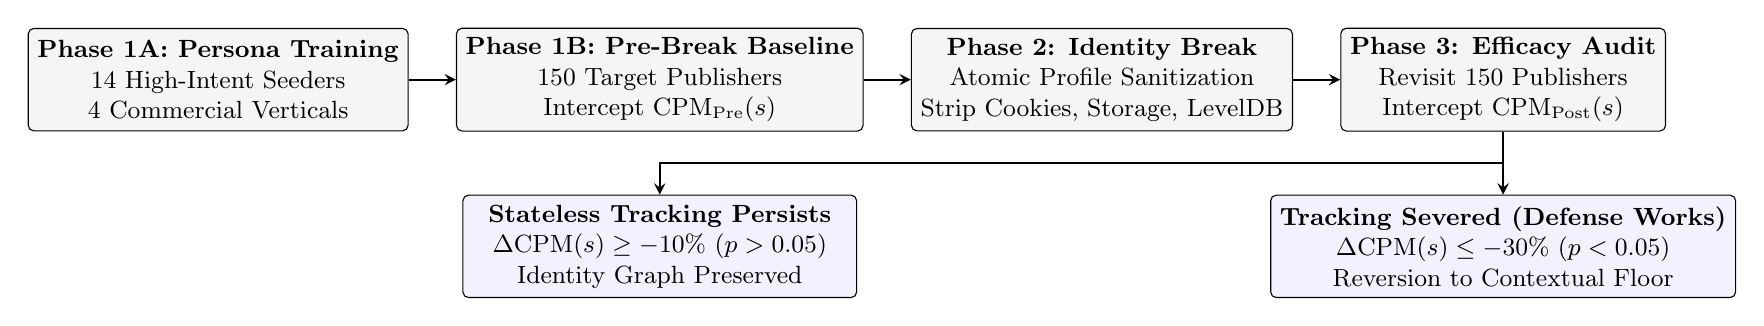
\begin{tikzpicture}[
    node distance=0.5cm and 0.6cm,
    phase/.style={draw, rectangle, rounded corners=2pt, minimum width=3.8cm, minimum height=1.3cm, align=center, fill=gray!8, font=\small},
    decision/.style={draw, rectangle, rounded corners=2pt, minimum width=5.0cm, minimum height=1.3cm, align=center, fill=blue!5, font=\small},
    arrow/.style={thick, ->, >=stealth}
]
    % Nodes
    \node (p1a) [phase] {\textbf{Phase 1A: Persona Training}\\14 High-Intent Seeders\\4 Commercial Verticals};
    \node (p1b) [phase, right=of p1a] {\textbf{Phase 1B: Pre-Break Baseline}\\150 Target Publishers\\Intercept $\cpm_{\text{Pre}}(s)$};
    \node (p2)  [phase, right=of p1b] {\textbf{Phase 2: Identity Break}\\Atomic Profile Sanitization\\Strip Cookies, Storage, LevelDB};
    \node (p3)  [phase, right=of p2] {\textbf{Phase 3: Efficacy Audit}\\Revisit 150 Publishers\\Intercept $\cpm_{\text{Post}}(s)$};

    % Causal Decision
    \node (dec1) [decision, below=0.8cm of p1b] {\textbf{Stateless Tracking Persists}\\$\Delta\cpm(s) \ge -10\%$ ($p > 0.05$)\\Identity Graph Preserved};
    \node (dec2) [decision, below=0.8cm of p3] {\textbf{Tracking Severed (Defense Works)}\\$\Delta\cpm(s) \le -30\%$ ($p < 0.05$)\\Reversion to Contextual Floor};

    % Paths
    \draw [arrow] (p1a) -- (p1b);
    \draw [arrow] (p1b) -- (p2);
    \draw [arrow] (p2) -- (p3);
    
    \draw [arrow] (p3.south) -- ++(0,-0.4) -| (dec1.north);
    \draw [arrow] (p3.south) -- ++(0,-0.4) -| (dec2.north);
\end{tikzpicture}
}
\caption{The 3-Phase Causal Measurement Lifecycle: Persona training ($t_0 \to t_1$), Pre-Break baseline capture ($t_1 \to t_2$), programmatic profile sanitization ($t_2 \to t_3$), and Post-Break re-crawl ($t_3 \to t_4$).}
\label{fig:causal_lifecycle}
\end{figure*}

\paragraph{Phase 1A: Persona Training ($t_0 \to t_1$)}
A fresh browser profile navigates across 14 high-value commercial seed domains structured across four high-yield advertising verticals: Financial \& Insurance, Automotive Research, Luxury Retail \& Lifestyle, and High-End Travel \& Real Estate (domain corpus detailed in Appendix~\ref{sec:appendix_seeders}). 
On each domain, the crawler resolves consent via the 3-Tier Consent Engine, dispatches hardware-level cursor movements, and waits for tracking pixels to register. 
This induces ad network identity entanglement~\cite{oh2022cart} and initializes cross-exchange retargeting profiles~\cite{bashir2016tracing}, establishing an ``Affluent Consumer'' persona in commercial device graphs.

\paragraph{Phase 1B: Pre-Break Baseline Measurement ($t_1 \to t_2$)}
Holding this persona, the browser navigates the 150 publisher targets. Upon reaching each domain, the crawler dispatches synthetic cursor events, resolves consent, and enforces a 15.0-second auction observation window to allow asynchronous Prebid bid adjustments to settle~\cite{cook2020inferring}. 
The network proxy intercepts clearing prices:
\begin{equation}
\cpm_{\text{Pre}}(s) = \max_{b \in \mathcal{B}_s} \{\cpm(b)\}
\end{equation}
where $\mathcal{B}_s$ is the set of all valid bids returned across active SSP adapters.

\paragraph{Phase 2: The Enforced Identity Break ($t_2 \to t_3$)}
The browser process is terminated, releasing file locks. The Atomic Profile Sanitizer removes all stateful storage primitives (cookies, web storage, cache partitions, and LevelDB journals; detailed in Appendix~\ref{sec:appendix_sanitizer})~\cite{whatwg_webstorage, acar2014web}, while strictly preserving client defensive configurations, flags, and certificates.

\paragraph{Phase 3: Efficacy Measurement ($t_3 \to t_4$)}
The sanitized browser revisits the exact same 150 publisher domains in identical order under the same network routing. The platform records the post-break clearing price:
\begin{equation}
\cpm_{\text{Post}}(s) = \max_{b \in \mathcal{B}_s'} \{\cpm(b)\}
\end{equation}
alongside runtime JavaScript exceptions and network tracking flows.

\subsection{Publisher Curation Pipeline}
\label{subsec:curation}

To ensure auctions are observable, publishers must run client-side header bidding rather than opaque server-side auctions~\cite{pachilakis2019no, cook2020inferring}. 
We curated $\mathcal{S}$ ($|\mathcal{S}| = 150$) from top Tranco ledger entries via a 4-stage filter:
\begin{enumerate}
    \item \textbf{TLD Selection:} Restrict domains to primary commercial English TLDs (\texttt{.com}, \texttt{.net}, \texttt{.org}, \texttt{.uk}, \texttt{.ca}, \texttt{.au}, \texttt{.nz}, \texttt{.ie});
    \item \textbf{Walled-Garden Elimination:} Filter out a 40-domain blacklist of platforms that monetize inventory exclusively through proprietary internal ad tech without OpenRTB (e.g., Google, Facebook, Amazon, Apple, Netflix, Wikipedia, StackOverflow);
    \item \textbf{Header Bidding Signature Detection:} Inspect landing-page source HTML for active wrappers (\texttt{prebid.js}, \texttt{pbjs.que}, \texttt{pubfood}, \texttt{apstag.js}, or \texttt{gpt.js});
    \item \textbf{Supply-Chain Validation (\texttt{ads.txt}):} Query \path{https://{domain}/ads.txt} and require an HTTP 200 status containing \texttt{"DIRECT"} authorized exchange relationships.
\end{enumerate}

\paragraph{The Paired Observability Filter ($\mathcal{S}_{\text{active}}$)}
Because production auctions can suffer transient exchange timeouts or dynamic allocation shifts, we enforce a strict Paired Observability Filter:
\begin{equation}
\mathcal{S}_{\text{active}}(c) = \left\{ s \in \mathcal{S} \;\middle|\; \cpm_{\text{Pre}}(s) > 0 \;\land\; \cpm_{\text{Post}}(s) > 0 \right\}
\end{equation}
Across configurations, $|\mathcal{S}_{\text{active}}|$ ranges from 33 to 54 domains ($22.0\%$ to $36.0\%$ transparency), ensuring that all calculated deltas represent valid, paired transactions. 
Workloads were parallelized across three Docker containers (50 domains/batch, 4\,GB shared memory) on dual Intel Xeon E5-2609 v4 and AMD EPYC 7343 nodes.

\subsection{Evaluated Browser Configurations}
\label{subsec:browser_matrix}

We evaluate five browser configurations across Blink and Gecko rendering engines:
\begin{enumerate}
    \item \textbf{\texttt{chrome\_baseline}:} Vanilla Google Chrome operating under default settings, acting as our unhardened control group;
    \item \textbf{\texttt{firefox\_baseline}:} Standard Mozilla Firefox with Enhanced Tracking Protection (ETP Standard);
    \item \textbf{\texttt{firefox\_hardened}:} Multi-layered hardened Firefox combining ETP Strict (\path{browser.contentblocking.category} = ``strict''), Total Cookie Protection (\path{network.cookie.cookieBehavior} = 5, dFPI), and query parameter stripping~\cite{randall2022measuring}. It also uses Tor-derived Resist Fingerprinting (\path{privacy.resistFingerprinting = true})~\cite{tor_design, torbrowser_normalization_2019, mozilla_rfp_docs};
    \item \textbf{\texttt{brave\_baseline}:} Standard Brave Browser with default Shields (Canvas and Audio Farbling enabled; standard network blocking)~\cite{brave_fingerprinting_protections_2025};
    \item \textbf{\texttt{brave\_hardened}:} Brave Browser with ``Strict'' Shields (farbling combined with aggressive network request blocking)~\cite{brave_fingerprinting_protections_2025}.
\end{enumerate}
\subsection{Metrics \& Econometric Ground Truth}
\label{subsec:metrics}

\paragraph{Relative Economic Bid Shift ($\Delta\cpm$)}
For each active domain $s \in \mathcal{S}_{\text{active}}$:
\begin{equation}
\Delta\cpm(s) = \frac{\cpm_{\text{Post}}(s) - \cpm_{\text{Pre}}(s)}{\cpm_{\text{Pre}}(s)}
\end{equation}

\paragraph{Econometric Resistance Thresholds}
Drawing on digital advertising econometric literature, we partition observed responses into three regimes:
\begin{itemize}
    \item \textbf{Tracked / Low Resistance ($\Delta\cpm \ge -10\%$):} RTB auctions display $5\%$--$10\%$ natural volatility from DSP budget pacing, time-of-day bid throttling, and latency fluctuations~\cite{barysei2023investigating}; shifts within this boundary indicate stateless identity persistence.
    \item \textbf{High Tracking Resistance ($\htr$, $\Delta\cpm \le -30\%$):} Behavioral targeting yields a documented $30\%$--$60\%+$ premium over untargeted contextual inventory~\cite{beales2014empirical, johnson2020consumer, google2019cookie}; drops exceeding $30\%$ indicate that cross-site behavioral tracking was disrupted.
    \item \textbf{Partial Resistance ($-30\% < \Delta\cpm < -10\%$):} Represents intermediate valuation, partial graph matching, or algorithmic bid shading.
\end{itemize}

\paragraph{Re-Identification Rate ($\rid$)}
The proportion of active publishers where the client is successfully re-identified:
\begin{equation}
\rid = \frac{\left| \{ s \in \mathcal{S}_{\text{active}} \mid \Delta\cpm(s) \ge -10\% \} \right|}{|\mathcal{S}_{\text{active}}|}
\end{equation}

\paragraph{Usability Cost ($\ucost$)}
Using the Site Breakage Index (SBI), runtime errors captured via our out-of-band logger are deduplicated by MD5 hashing normalized error strings and stack locations ($U_e$). 
To account for cross-engine variations between Gecko and Blink, we normalize against the control group (\texttt{chrome\_baseline}):
\begin{equation}
\ucost = \max\left(0.0,\; \frac{U_e(\text{Test}) - U_e(\text{Chrome})}{U_e(\text{Chrome})}\right)
\end{equation}
where excess exceptions reflect broken DOM dependency chains triggered by blocked tracking endpoints~\cite{iqbal2020adgraph}.

\subsection{Statistical Hypothesis Testing}
\label{subsec:stats}

Because auction prices follow right-skewed, heavy-tailed distributions with left-censored reserve floors, parametric tests are invalid~\cite{barysei2023investigating}. We apply the non-parametric \textbf{Paired Wilcoxon Signed-Rank Test}:
\begin{equation}
H_0: \text{median}(\Delta\cpm) = 0 \quad \text{vs.} \quad H_1: \text{median}(\Delta\cpm) < 0
\end{equation}
calculated over the signed ranks of non-zero absolute differences $|D_s| = |\cpm_{\text{Post}}(s) - \cpm_{\text{Pre}}(s)|$. 

Following the American Statistical Association guidelines on statistical inference~\cite{wasserstein2016asa}, we interpret non-parametric rank tests in conjunction with real-world effect sizes ($\Delta\cpm$). 
To test whether the five browser configurations diverge systematically across the complete parameter space, we compute an omnibus \textbf{Kruskal-Wallis test} across all groups. With the causal protocol and econometric thresholds established, we deploy this experimental design to evaluate the empirical performance of each defense configuration.
\section{Empirical Evaluation}
\label{sec:evaluation}

Operating our causal measurement platform across all five browser configurations, our testbed completed crawls over all 150 curated publisher domains across both phases ($100.0\%$ completion yield). 
Table~\ref{tab:master_results} presents the empirical results structured across our three measurement silos: economic bid valuation, network identity diffusion, and client-side usability overheads.

\begin{table*}[t]
\centering
\small
\caption{Master Empirical Evaluation Matrix across 150 Commercial Publishers. 
Absolute bids reflect Pre/Post medians; $\Delta\cpm$ distributions show first quartile ($Q_1$), median, and third quartile ($Q_3$); Identity Diffusion decomposes into Cookie Syncs ($S_{\text{post}}$) and Smuggled UIDs ($U_{\text{post}}$); Usability Cost ($\ucost$) is normalized to the Chrome control group.}
\label{tab:master_results}
\resizebox{\textwidth}{!}{%
\setlength{\tabcolsep}{4pt}
\begin{tabular}{lcccccccccccc}
\toprule
\textbf{Configuration} & $|\mathcal{S}_{\text{active}}|$ & \textbf{Pre \$} & \textbf{Post \$} & $\rid$ & \textbf{Spread ($Q_1$ / Med / $Q_3$)} & \textbf{IQR} & $S_{\text{post}}$ & $U_{\text{post}}$ & $D_{\text{ID}}$ & $\ucost$ & \textbf{Wilcoxon $W$ ($p$)} & $\etr$ \\
\midrule
\texttt{chrome\_baseline}  & 33 & \$0.08 & \$0.05 & 0.606 & -75.00\% / \textbf{-1.12\%} / +123.11\% & 198.11\% & 3,206 & 18,359 & 21,565 & 0.00 & 226.5 ($p=0.4832$) & 0.105 \\
\texttt{firefox\_baseline} & 46 & \$0.09 & \$0.05 & 0.543 & -99.30\% / \textbf{-4.11\%} / +106.19\% & 205.49\% & 2,461 & 18,414 & 20,875 & 0.00 & 414.0 ($p=0.3445$) & 0.136 \\
\texttt{brave\_baseline}   & 41 & \$0.15 & \$0.08 & 0.537 & -100.0\% / \textbf{-21.39\%} / +46.95\% & 146.95\% & 3,302 & 18,515 & 21,817 & 0.31 & 345.0 ($p=0.5300$) & 0.131 \\
\texttt{firefox\_hardened} & 54 & \$0.09 & \textbf{\$0.02} & 0.574 & -99.86\% / \textbf{-26.86\%} / \textbf{+1.20\%} & 101.06\% & 6,006 & 22,970 & 28,976 & 0.00 & 472.0 ($p=\textbf{0.0734}$) $\dagger$ & 0.175 \\
\texttt{brave\_hardened}   & 46 & \$0.15 & \textbf{\$0.06} & \textbf{0.500} & -100.0\% / \textbf{-59.98\%} / \textbf{0.00\%} & \textbf{100.00\%} & 3,229 & 18,885 & 22,114 & \textbf{0.44} & 361.5 ($p=0.1192$) & \textbf{0.179} \\
\bottomrule
\end{tabular}%
}
\vspace{1pt}
\flushleft{\footnotesize $\dagger$ Statistically significant at the marginal $\alpha = 0.10$ level. Omnibus Kruskal-Wallis across all 5 configurations: $H = 7.570$, $p = 0.1087$.}
\end{table*}

\subsection{Dataset Integrity \& CMP Consent Yield}
\label{subsec:observability_yield}

Applying the Paired Observability Filter (Section~\ref{subsec:curation}) extracted between 33 and 54 actively observable publisher auctions per configuration ($22.0\%$ to $36.0\%$ Prebid transparency). 

As established in prior header bidding measurements~\cite{pachilakis2019no, cook2020inferring}, client-side wrappers capture the observable portion of programmatic inventory; unobserved domains either route auctions through opaque Server-to-Server (S2S) frameworks (e.g., Google Open Bidding, Amazon TAM) or experienced exchange timeouts exceeding our 15.0-second collection window. 

Crucially, the 3-Tier Consent Clicker successfully negotiated European privacy gates across the crawl:
\begin{itemize}
    \item \texttt{chrome\_baseline}: 107 domains resolved ($71.3\%$ auto-accepted; 61 regex, 43 CSS, 3 API);
    \item \texttt{firefox\_hardened}: 118 domains resolved ($78.7\%$ auto-accepted; 64 regex, 53 CSS, 1 API);
    \item \texttt{brave\_hardened}: 114 domains resolved ($76.0\%$ auto-accepted; 59 regex, 51 CSS, 4 API).
\end{itemize}
The unhandled minority ($21.3\%$--$32.0\%$) comprised non-EU sites lacking consent banners or publishers serving custom, non-standard modal overlays~\cite{papadogiannakis2021user}.

\subsection{Silo 1: Economic Valuation Analysis}
\label{subsec:silo_econ}

Figure~\ref{fig:iqr_spread} plots the full distributional spread of relative bid shifts across configurations, demonstrating how defensive hardening compresses market valuation.

\begin{figure}[t]
\centering
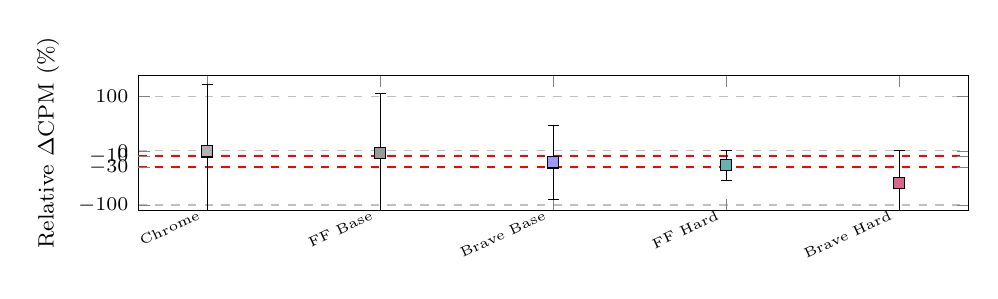
\begin{tikzpicture}
\begin{axis}[
    width=\columnwidth,
    height=3.3cm,
    ymin=-110, ymax=140,
    ylabel={Relative $\Delta\cpm$ (\%)},
    ylabel style={font=\footnotesize},
    ticklabel style={font=\scriptsize},
    symbolic x coords={Chrome, FF Base, Brave Base, FF Hard, Brave Hard},
    xtick={Chrome, FF Base, Brave Base, FF Hard, Brave Hard},
    x tick label style={rotate=25, anchor=east, font=\tiny},
    ymajorgrids=true,
    grid style=dashed,
    extra y ticks={-10, -30},
    extra y tick style={grid=major, grid style={red, dashed, line width=0.8pt}}
]
% Box plots via error bars: Q1 to Q3, with median marks
\addplot+[black, mark=square*, mark options={fill=gray!60}, error bars/.cd, y dir=both, y explicit] 
    coordinates {(Chrome, -1.12) +- (73.88, 124.23)};
\addplot+[black, mark=square*, mark options={fill=gray!80}, error bars/.cd, y dir=both, y explicit] 
    coordinates {(FF Base, -4.11) +- (95.19, 110.30)};
\addplot+[black, mark=square*, mark options={fill=blue!40}, error bars/.cd, y dir=both, y explicit] 
    coordinates {(Brave Base, -21.39) +- (78.61, 68.34)};
\addplot+[black, mark=square*, mark options={fill=teal!60}, error bars/.cd, y dir=both, y explicit] 
    coordinates {(FF Hard, -26.86) +- (73.00, 28.06)};
\addplot+[black, mark=square*, mark options={fill=purple!60}, error bars/.cd, y dir=both, y explicit] 
    coordinates {(Brave Hard, -59.98) +- (40.02, 59.98)};
\end{axis}
\end{tikzpicture}
\caption{Distributional spread of relative price shifts ($\Delta\cpm$) across configurations. Points indicate median values; error bars denote the Interquartile Range ($Q_1$ to $Q_3$). Red dashed lines indicate the $-10\%$ noise and $-30\%$ \htr boundaries.}
\label{fig:iqr_spread}
\end{figure}

\paragraph{Negative Control \& Default Defenses}
In unhardened Chrome, state purging produces a median bid shift of only $-1.12\%$ ($p = 0.4832$, fail to reject $H_0$), with $60.61\%$ of publishers re-identifying the client within market noise ($\rid = 0.606$). 
While isolated domains experience bid drops (e.g., \url{allrecipes.com}, $\$10.00 \to \$0.00$), others clear at elevated rates (e.g., \url{archdaily.com}, $\$26.00$), demonstrating empirically that commercial DSPs routinely bridge storage resets via stateless graphs~\cite{acar2014web, liu2025first}. 
Default browser protections offer negligible resistance: standard Firefox yields a median shift of $-4.11\%$ ($p = 0.3445$, $\rid = 0.543$), as static ETP blocklists fail to restrict active canvas or audio readbacks. 
While default Brave farbling induces valuation uncertainty ($\Delta\cpm = -21.39\%$, median $\$0.15 \to \$0.08$) through algorithmic bid shading~\cite{barysei2023investigating}, its wide dispersion ($Q_3 = +46.95\%$, $\rid = 0.537$) confirms that cross-session graph linkage remains largely intact.

\paragraph{Hardened Defenses: Normalization vs.\ Disruption}
Hardened configurations alter auction dynamics substantially, establishing two distinct operational profiles. Hardened Firefox achieves a $-26.86\%$ median bid collapse ($p = 0.0734$, $W = 472.0$), driving the median clearing bid from $\$0.09$ down to $\$0.02$ ($77.8\%$ decline) with the upper quartile compressed to $Q_3 = +1.20\%$. 
Crucially, Tor-derived RFP normalization achieves this disruption with zero client-side script breakage ($\ucost = 0.00$). In contrast, Hardened Brave enforces the most aggressive economic intervention: median bids collapse by $-59.98\%$ ($\$0.15 \to \$0.06$, $\rid = 0.500$). 
Its lower quartile drops to complete bid suppression ($Q_1 = -100.0\%$, with domains like \url{dailymail.co.uk} and \url{cricbuzz.com} falling to $\$0.00$), while the upper quartile is capped at $Q_3 = 0.00\%$, indicating non-positive bid shifts across $75\%$ of active inventory. 
However, this tracking severance comes at the expense of severe script dependency breakage ($\ucost = 0.44$).

\subsection{Ad-Tech Pricing \& Non-Parametric Rank Dilution}
\label{subsec:rank_dilution}

Despite Brave Hardened's $-59.98\%$ median collapse and $Q_3 \le 0.00\%$ compression, its paired Wilcoxon test yielded $W = 361.5$ ($p = 0.1192$). 
This statistical artifact stems from two structural properties of programmatic ad markets~\cite{barysei2023investigating}: 
(1)~\textit{Left-censored reserve floors} ($\$0.01$--$\$0.05$) truncate negative differences ($|D_i| \le \$0.15$); and 
(2)~\textit{heteroskedastic video outliers} heavily penalize signed-rank sums. 
Because the Wilcoxon test ranks observations by absolute dollar difference ($|D_i|$), isolated outstream video ad spikes (e.g., $\$0.04 \to \$16.00$ on \url{standard.co.uk}, and $\$0.10 \to \$22.00$ on \url{verywellhealth.com}) receive maximum ranks ($R_i = N$), counterbalancing dozens of consistent display ad collapses ($-\$0.50$). 
Per ASA inference guidelines~\cite{wasserstein2016asa}, real-world economic significance in high-variance financial auctions must be evaluated via effect size and quartile compression ($Q_3 \le 0.00\%$) rather than rank-sum symmetry alone.

\subsection{Silo 2: Identity Diffusion \& The Retry Storm}
\label{subsec:silo_network}

While clearing prices reveal identity certainty from the buyer's perspective, inspecting underlying network flows demonstrates how browser defenses alter tracker coordination in the background.
Decomposing Identity Diffusion ($D_{\text{ID}}$) into Cookie Synchronizations ($S_{\text{post}}$)~\cite{papadopoulos2019cookie} and Smuggled Navigational Identifiers ($U_{\text{post}}$)~\cite{randall2022measuring} reveals an unexpected operational divergence across configurations:
Across \texttt{chrome\_baseline}, \texttt{firefox\_baseline}, and both Brave configurations, syncs and smuggled UIDs remained remarkably stable: $S_{\text{post}} \in [2,461, 3,302]$ and $U_{\text{post}} \in [18,359, 18,885]$.
In stark contrast, \texttt{firefox\_hardened} exhibited a pronounced surge: \textbf{Cookie Synchronizations more than doubled to $S_{\text{post}} = 6,006$}, and \textbf{Smuggled UIDs surged to $U_{\text{post}} = 22,970$}, driving total diffusion events to $D_{\text{ID}} = 28,976$. 
Inspection of proxy logs reveals this was driven by a \textbf{stateless blocking retry storm}: when Firefox's multi-layered defenses (Total Cookie Protection, RFP canvas blanking, and query parameter stripping) blocked tracker endpoints and sanitized link decorations, client-side tracking scripts threw exceptions and repeatedly re-triggered synchronization requests within recursive event loops~\cite{iqbal2020adgraph}. 
Crucially, deduplicating target endpoints revealed that Hardened Firefox communicated with the fewest distinct tracking hosts (\textbf{810 hosts}, vs. 872 in Chrome and 888 in Brave Hardened). Thus, while request \textbf{frequency} spiked due to client-side retries, Firefox successfully restricted the \textbf{diffusion} of identifiers across unique commercial entities.

\subsection{Silo 3: Usability Cost \& Runtime Breakage}
\label{subsec:silo_usability}

While normalized defenses contained entity diffusion without modifying DOM layouts, blocking network requests introduced measurable client-side breakage.

Client-side error logging captured 45,000+ unhandled runtime JavaScript exceptions across our crawls. Cross-engine normalization reveals key differences between defense approaches:
\begin{itemize}
    \item \textbf{Gecko Engine Performance:} Standard Firefox recorded 1,590 exceptions, while Hardened Firefox recorded 2,400 exceptions ($+50.9\%$). 
However, because RFP's timer quantization and canvas blanking return syntactically valid mock objects, these errors did not alter DOM layout trees or break page scripts, preserving a usability penalty of $\ucost = 0.00$.
    \item \textbf{Chromium Engine Performance:} Chrome Baseline recorded 12,816 exceptions. Brave Baseline logged 13,309 exceptions ($\ucost = 0.31$), and Brave Hardened logged 14,882 exceptions ($\ucost = 0.44$).
\end{itemize}

Brave's aggressive network-layer request blocking severs script dependency chains, causing downstream publisher scripts to throw unhandled \texttt{TypeError} and null-pointer exceptions that degrade site features~\cite{iqbal2020adgraph}. 
These empirical results reveal an operational paradox: defensive blocking triggers network retry storms that artificially inflate raw request counts, while aggressive filtering incurs substantial usability breakage. In Section~\ref{sec:discussion}, we deconstruct how naive composite metrics fail to capture these trade-offs, motivating the formulation of $\etr$.
\section{Discussion: The Usability Trap \& Metric Refinement}
\label{sec:discussion}

The interplay between identity disruption, network containment, and client breakage exposes structural deficiencies in naive privacy-usability metrics. 
Here, we deconstruct the failure of our initial metric formulation, present the axiomatic derivation of the Refined Effectiveness-to-Risk metric ($\etr$), and map the empirical Pareto frontier governing browser privacy.

\subsection{Deconstructing the Usability Trap}
\label{subsec:usability_trap}

Initial privacy measurement frameworks often model the trade-off between tracking mitigation and usability via intuitive composite quotients. We initially benchmarked browser configurations using the formulation:
\begin{equation}
\etrinit = \frac{(1 - \rid) \times \left( \frac{1}{\ln(D_{\text{ID}} + e)} \right)}{1 + \ucost}
\label{eq:etr_initial}
\end{equation}
Evaluating our empirical corpus under Equation~\ref{eq:etr_initial} produced an anomalous, inverted ranking:
\begin{align*}
\etrinit: \; & \text{FF Base (0.046)} > \text{FF Hard (0.042)} > \text{Chrome (0.040)} \\
& > \text{Brave Base (0.035)} > \text{Brave Hard (0.035)}
\end{align*}
This formulation ranked completely unhardened Chrome ($0.0395$) \textit{higher} than Brave Hardened ($0.0347$), despite the latter destroying $60\%$ of auction clearing revenue and capping the upper quartile at $Q_3 = 0.00\%$. 
Forensic analysis revealed three mathematical pathologies:

\paragraph{1. Binary Disruption Insensitivity}
The binary re-identification rate $\rid$ registers an active domain as ``tracked'' if $\Delta\cpm \ge -10\%$. This threshold creates a step-function discontinuity that ignores deep economic disruption: a minor drop of $-11\%$ is treated identically to complete market annihilation ($-100.0\%$). 
Consequently, Brave Hardened's median collapse ($-59.98\%$) and $25\%$ total wipeout rate were completely discarded by the numerator.

\paragraph{2. Linear Denominator Penalty}
The linear denominator ($1 + \ucost = 1.44$) penalized Brave Hardened by $44\%$, disproportionately degrading its score and drowning out its substantial privacy gains.

\paragraph{3. The Retry-Storm Inversion}
Equation~\ref{eq:etr_initial} uses raw identity diffusion events ($D_{\text{ID}}$) in the logarithmic denominator. As revealed in Section~\ref{subsec:silo_network}, blocking tracker endpoints triggers client-side retry storms: client scripts repeatedly re-trigger cookie synchronization~\cite{papadopoulos2019cookie} and UID decoration loops~\cite{randall2022measuring} within recursive event handlers~\cite{iqbal2020adgraph}. 
This paradoxically inflated Hardened Firefox's diffusion volume to 28,976 total events (6,006 cookie syncs and 22,970 smuggled UIDs), penalizing the browser for effectively blocking third-party endpoints.

\subsection{Axiomatic Formulation of $\etr$}
\label{subsec:etr_star}

To resolve these distortions, we formulate the \textbf{Refined Effectiveness-to-Risk Metric} ($\etr$):
\begin{equation}
\etr = \frac{\Phi_{\text{econ}} \times \Psi_{\text{containment}}}{\Omega_{\text{usability}}}
\label{eq:etr_refined}
\end{equation}
where each component satisfies strict axiomatic requirements:

\paragraph{Continuous Economic Disruption ($\Phi_{\text{econ}}$)}
We replace the binary factor $(1 - \rid)$ with a composite economic index that integrates binary resistance, high-tier disruption, and median price decay:
\begin{equation}
\Phi_{\text{econ}} = \frac{(1 - \rid) + \htr + \max(0, -\widetilde{\Delta\cpm})}{3}
\end{equation}
where $\widetilde{\Delta\cpm}$ is the median relative bid shift. $\Phi_{\text{econ}} \in [0, 1]$ scales monotonically with both the breadth ($\htr$) and depth ($-\widetilde{\Delta\cpm}$) of tracking disruption.

\paragraph{Entity Density Containment ($\Psi_{\text{containment}}$)}
To eliminate retry-storm artifacts, we replace raw request counts with the density of unique tracking entities contacted per publisher:
\begin{equation}
\Psi_{\text{containment}} = \frac{1}{\ln\left(\frac{D_{\text{entity}}}{N_{\text{sites}}} + e\right)}
\end{equation}
where $D_{\text{entity}}$ is the count of deduplicated third-party hosts and $N_{\text{sites}} = 150$. By evaluating host density ($d = D_{\text{entity}} / 150$), $\Psi$ rewards browsers that restrict communication across distinct corporate tracking entities~\cite{bashir2016tracing, cook2020inferring}, remaining invariant to local script retry loops. As $D_{\text{entity}} \to 0$, $\Psi \to 1.0$.

\paragraph{Sub-Linear Usability Dampening ($\Omega_{\text{usability}}$)}
To prevent script exceptions from disproportionately penalizing privacy gains, we dampen the usability penalty logarithmically:
\begin{equation}
\Omega_{\text{usability}} = 1 + \ln(1 + \ucost)
\end{equation}
This dampens the impact of script errors, ensuring that browsers achieving deep privacy protection are not penalized below unhardened baselines.

\begin{table}[t]
\centering
\small
\caption{Decomposition of Refined Metric Components ($\etr$). Deduplicated tracking host density restores monotonically sound defense rankings.}
\label{tab:etr_breakdown}
\resizebox{\columnwidth}{!}{%
\begin{tabular}{lcccccc}
\toprule
\textbf{Configuration} & $\Phi_{\text{econ}}$ & $\frac{D_{\text{entity}}}{N}$ & $\Psi_{\text{cont}}$ & $\Omega_{\text{use}}$ & $\etr$ & \textbf{Rank} \\
\midrule
\texttt{chrome\_baseline}  & 0.226 & 5.813 & 0.467 & 1.000 & \textbf{0.105} & Control \\
\texttt{firefox\_baseline} & 0.289 & 5.613 & 0.471 & 1.000 & \textbf{0.136} & Dominated \\
\texttt{brave\_baseline}   & 0.322 & 5.760 & 0.468 & 1.270 & \textbf{0.131} & Dominated \\
\texttt{firefox\_hardened} & 0.368 & \textbf{5.400} & \textbf{0.476} & 1.000 & \textbf{0.175} & Pareto Apex \\
\texttt{brave\_hardened}   & \textbf{0.526} & 5.920 & 0.465 & 1.365 & \textbf{0.179} & Pareto Apex \\
\bottomrule
\end{tabular}%
}
\end{table}

\paragraph{Benchmark Restoration}
As demonstrated in Table~\ref{tab:etr_breakdown}, $\etr$ restores a consistent ranking:
\begin{align*}
\etr: \;\; & \text{Brave Hard (0.179)} > \text{FF Hard (0.175)} > \text{FF Base (0.136)} \\
& > \text{Brave Base (0.131)} > \text{Chrome Base (0.105)}
\end{align*}
Unhardened Chrome correctly anchors the bottom of the benchmark, while Hardened Brave and Hardened Firefox share the upper bound through complementary trade-offs.

\subsection{The Empirical Pareto Frontier}
\label{subsec:pareto_frontier}

Our empirical findings demonstrate that client-side web privacy adheres to a multi-objective Pareto optimization problem: maximizing economic tracking disruption ($\Phi_{\text{econ}}$) while minimizing usability breakage ($\ucost$).

\begin{figure}[t]
\centering
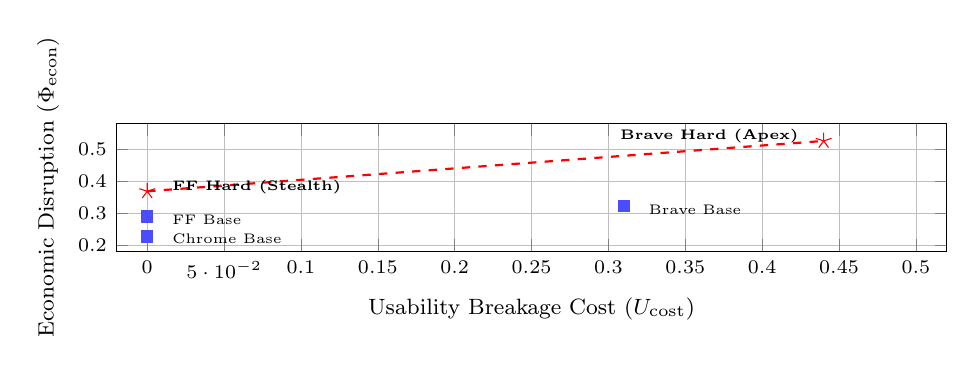
\begin{tikzpicture}
\begin{axis}[
    width=\columnwidth,
    height=3.2cm,
    xlabel={Usability Breakage Cost ($\ucost$)},
    ylabel={Economic Disruption ($\Phi_{\text{econ}}$)},
    xlabel style={font=\footnotesize},
    ylabel style={font=\footnotesize},
    ticklabel style={font=\scriptsize},
    xmin=-0.02, xmax=0.52,
    ymin=0.18, ymax=0.58,
    grid=both,
    grid style={line width=.1pt, draw=gray!20},
    major grid style={line width=.2pt,draw=gray!50}
]

% Pareto Frontier Line
\addplot[thick, dashed, red] coordinates {
    (0.00, 0.368) % FF Hard
    (0.44, 0.526) % Brave Hard
};

% Non-dominated Pareto Optimal Points
\addplot[only marks, mark=star, mark size=3.0pt, red] coordinates {
    (0.00, 0.368) % FF Hardened
    (0.44, 0.526) % Brave Hardened
};

% Dominated Points
\addplot[only marks, mark=square*, mark size=2.0pt, blue!70] coordinates {
    (0.00, 0.226) % Chrome
    (0.00, 0.289) % FF Base
    (0.31, 0.322) % Brave Base
};

% Labels with manual offset to avoid margin collision
\node[anchor=west, font=\tiny] at (axis cs:0.01,0.38) {\textbf{FF Hard (Stealth)}};
\node[anchor=east, font=\tiny] at (axis cs:0.43,0.54) {\textbf{Brave Hard (Apex)}};
\node[anchor=west, font=\tiny] at (axis cs:0.01,0.22) {Chrome Base};
\node[anchor=west, font=\tiny] at (axis cs:0.01,0.28) {FF Base};
\node[anchor=west, font=\tiny] at (axis cs:0.32,0.31) {Brave Base};

\end{axis}
\end{tikzpicture}
\caption{The Empirical Privacy-Usability Pareto Frontier. The red dashed line connects the non-dominated Pareto boundaries: Stealth Optimum (FF Hardened) and Apex Disruption (Brave Hardened).}
\label{fig:pareto}
\end{figure}

As mapped in Figure~\ref{fig:pareto}, defense strategies define an empirical frontier:
\begin{enumerate}
    \item \textbf{The Stealth / Zero-Breakage Optimum (\texttt{firefox\_hardened}):} Combining Tor-derived API normalization (RFP)~\cite{tor_design, mozilla_rfp_docs} with Total Cookie Protection and query stripping~\cite{randall2022measuring} achieves $\Phi_{\text{econ}} = 0.368$ (a $-26.86\%$ median bid collapse) with \textbf{zero usability breakage ($\ucost = 0.00$)}. 
    Because RFP normalizes API return values to uniform mock pools rather than severing network calls, downstream publisher code continues executing cleanly.
    \item \textbf{The Maximum Privacy Optimum (\texttt{brave\_hardened}):} Combining API farbling~\cite{brave_fingerprinting_protections_2025} with aggressive network-level blocking maximizes tracking severance ($\Phi_{\text{econ}} = 0.526$, $-59.98\%$ median collapse, $\rid = 0.500$), but incurs $\ucost = 0.44$ due to severed script dependency chains~\cite{iqbal2020adgraph}. 
    \item \textbf{Dominated Configurations:} \nolinkurl{chrome_baseline}, \nolinkurl{firefox_baseline}, and \nolinkurl{brave_baseline} are strictly Pareto-dominated, yielding weaker privacy protections without offering offsetting usability advantages.
\end{enumerate}

\subsection{Methodological Post-Mortem}
\label{subsec:post_mortem}

During platform validation, we identified a critical experimental failure mode: naive filesystem profile cloning leaked persistent identifiers across phases. 
Chromium caches session descriptors and HSTS tokens within binary LevelDB transaction logs and service worker quotas. In early test runs, unpurged LevelDB files preserved cross-phase identity state, producing artificial $0.0\%$ bid shifts.

This failure confirms empirical findings by Acar et al.~\cite{acar2014web} and Lerner et al.~\cite{lerner2016internet}, who demonstrated that commercial tracking networks exploit persistent HTML5 Web Storage~\cite{whatwg_webstorage} and HSTS supercookies to respawn deleted identifiers. 
Standard browser ``Clear Browsing Data'' routines are insufficient for rigorous web measurement; reliable causal interventions require deterministic profile sanitization that wipes underlying LevelDB stores while preserving anti-fingerprinting defenses.
\section{Limitations}
\label{sec:threats}

\paragraph{Client-Side vs.\ Server-Side Bidding}
Our causal oracle intercepts client-side \texttt{Prebid.js} auctions. While client-side bids reflect direct market demand, proprietary Server-to-Server (S2S) frameworks (e.g., Google Open Bidding, Amazon TAM) remain opaque behind publisher ad servers~\cite{pachilakis2019no, cook2020inferring}.

\paragraph{Usability Proxy: Exception Overhead}
We quantify usability cost via normalized runtime JavaScript exceptions ($\ucost$). While exceptions capture severed script dependencies and broken execution graphs~\cite{iqbal2020adgraph}, they are an indirect proxy for functional failure. 
We treat $\ucost$ as a reproducible initial baseline and encourage the community to propose alternative methodologies (e.g., visual layout shifts or synthetic user journey completion rates) to standardize web breakage benchmarks.

\paragraph{Synthetic Personas vs.\ Longitudinal Drift}
Our 14-seeder profiles initialize commercial DSP device graphs and trigger premium bid pacing~\cite{bashir2016tracing, oh2022cart}, but lack the longitudinal entropy of multi-month human browsing (e.g., latent logins and search histories)~\cite{zeber2020representativeness, lerner2016internet}.

\paragraph{Software Rasterization Trade-offs}
Mesa software rasterization (\texttt{swrast}) enforced determinism across cluster workers and eliminated GPU confounding, though commercial scripts may probe bare-metal GPU driver signatures~\cite{mowery2012pixel, cao2017cross} that software rasterization inherently normalizes.

\paragraph{Geographic Vantage}
Workloads operated from European academic IPs (Portugal); GDPR and ePrivacy enforcement may induce distinct bid density and consent gating compared to non-GDPR regions~\cite{papadogiannakis2021user, barysei2023investigating}.
\section{Conclusion}
\label{sec:conclusion}

This paper presented the first outcome-oriented, causal measurement framework evaluating modern anti-fingerprinting defenses through programmatic Real-Time Bidding clearing prices. 
Across 150 commercial publishers, our experiments proved that stateful profile clearing alone is ineffective against modern ad tech: unhardened Chrome exhibited an imperceptible $-1.12\%$ bid drop ($p = 0.4832$), confirming that commercial Demand-Side Platforms routinely bypass storage resets using stateless fingerprinting~\cite{acar2014web, liu2025first}.

Conversely, anti-fingerprinting defenses disrupt commercial tracking along an empirical Pareto frontier:
(1)~\textbf{Hardened Firefox} achieves the \textit{Stealth / Zero-Breakage Optimum}, delivering a $-26.86\%$ median bid collapse ($p = 0.0734$) and superior host containment (810 hosts) with zero runtime script breakage ($\ucost = 0.00$); and
(2)~\textbf{Hardened Brave} achieves the \textit{Apex Disruption Optimum}, collapsing median bids by $-59.98\%$ ($Q_3 \le 0.00\%$), but at the cost of a $+44\%$ surge in runtime script breakage ($\ucost = 0.44$).

Finally, our formulation of the Refined Effective Tracking Resistance metric ($\etr$) resolves the ``Usability Trap,'' proving that defensive request blocking triggers tracker retry loops that invert naive evaluation metrics. 
To prevent script breakage while preserving user privacy, browser vendors should transition from aggressive network blocking toward API normalization and mock-return shims~\cite{iqbal2020adgraph, tor_design}. In accordance with web measurement reproducibility standards~\cite{demir2022reproducibility}, we open-source our testbed and auction datasets to foster reproducible research in web privacy.

% Balance columns on final page of body
\balance

% References (Does not count against the 8-page body limit)
\bibliographystyle{ACM-Reference-Format}
\bibliography{references}

% Optional Appendix (Pages 9-12)
\appendix
\section{Atomic Profile Sanitizer Implementation}
\label{sec:appendix_sanitizer}

During preliminary test crawls, standard profile cloning routines leaked persistent state across phases. Specifically, Blink- and Gecko-based browsers maintain internal LevelDB transaction journals, HTTP Strict Transport Security (HSTS) state caches, and persistent Service Worker registrations that survive standard cookie-clearing routines~\cite{acar2014web, whatwg_webstorage}. When profiles were copied naively between Phase 1B and Phase 3, these background stores re-hydrated tracking tokens, resulting in artificial $0.0\%$ bid shifts.

To ensure a provably clean storage state while preserving client defense configurations (e.g., Brave Shield levels, Firefox \path{about:config} preferences, and installed extension certificates), the platform executes an \textbf{Atomic Profile Sanitizer}. 

Before Phase 3 initializes, the orchestrator terminates the browser process, waits for operating system file locks to clear, and replicates the user profile directory while enforcing strict directory and file exclusion patterns via Python's \texttt{shutil}:

\begin{small}
\begin{verbatim}
EXCLUDED_PATTERNS = shutil.ignore_patterns(
    'SingletonLock', 'SingletonSocket', 'SingletonCookie',
    'parent.lock', 'lock', '.parentlock',
    'Cookies*', 'Cache*', 'Local Storage', 
    'IndexedDB', 'Session Storage', 'Sessions',
    'Network Persistent State', 'TransportSecurity',
    'QuotaManager', 'Service Worker', 'shared_proto_db',
    'BrowserMetrics*', 'Crashpad'
)
\end{verbatim}
\end{small}

Furthermore, for Firefox configurations, the sanitizer extracts and purges ephemeral SQLite identity stores (\path{cert9.db}, \path{key4.db}, \path{pkcs11.txt}) before injecting fresh sidecar certificates. This ensures that post-break browser profiles initialize from a completely clean storage slate while maintaining exact defensive configurations.

\end{document}